\begin{figure*}[t]
\centering
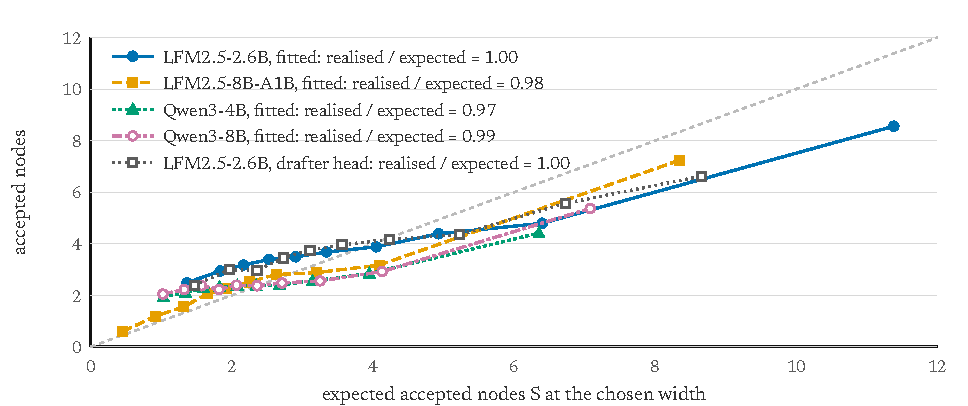
\includegraphics[width=0.8\textwidth]{gen/fig-calibration-img.pdf}
\caption{Accepted nodes per round against the expected accepted nodes $S$ at the chosen width, in ten equal-count bins of $S$ per series, on the instrumented run over the short subset, over the rounds whose width the chooser set from $S$ (cold-start rounds have none). The dashed diagonal is perfect calibration. Realised over expected accepted nodes: LFM2.5-2.6B, fitted 0.997 (1,460 rounds); LFM2.5-8B-A1B, fitted 0.981 (1,998 rounds); Qwen3-4B, fitted 0.973 (3,208 rounds); Qwen3-8B, fitted 0.986 (3,972 rounds); LFM2.5-2.6B, drafter head 1.004 (1,642 rounds). The drafter-head series is the cost-model arm, which prices the tree with the head-based estimate.}
\label{fig:calibration}
\end{figure*}
